\documentclass[11pt]{article}
\usepackage{geometry}
\geometry{letterpaper, margin=1in}
\usepackage[utf8]{inputenc}
\usepackage{graphicx}
\usepackage{upgreek}
\usepackage{url}
\usepackage[T1]{fontenc}
\usepackage{amsmath}
\usepackage{minted}
\usepackage{scalerel}
\usepackage{hyperref}
\usepackage[colorinlistoftodos]{todonotes}
\usepackage[
backend=biber,
style=ieee,
sorting=none
]{biblatex}
 
\addbibresource{refs.bib}

\title{ECE532S Digital Systems Design \\ \vspace{0.4cm}
       \Large Tutorial 3 - Adding Memory to the Microblaze Project \\ \vspace{0.4cm}
       \small Last Updated: July, 2019}
\author{ }
\date{ }


\begin{document}
\maketitle
\vspace{-1cm}

In this tutorial, we build a MicroBlaze-based system similar to the one built in the previous tutorial, but we also include a connection from the processor to some additional memory (separate from the program memory instantiated by the \textit{automated block connection}). In the previous design, the MicroBlaze was connected to a program and data Block RAM (BRAM) through the \textit{Local Memory Bus} connection interface standard. This connection allows for fast access to BRAM memory from the MicroBlaze, but this memory is not shareable with other cores in our system. If we'd like to have a memory that is accessible from the MicroBlaze and some other core in our system, we usually rely on the \textit{AXI} connection interface standard. The \textit{AXI} standard explicitly allows multiple masters (devices that can issue read and write requests) and is commonly used in industry.

For this tutorial, we will show how to connect a microblaze to an AXI-based memory. In the first part of the tutorial, this memory will take the form of a BRAM, which recall from the previous tutorial is an SRAM-based memory available within the logic of the FPGA. Next, we will replace this BRAM memory with an AXI-based \textit{memory controller} that can connect to the DDR memory on the Nexsys board (a 128 MB Micron MT47H64M16HR-25 DDR2 module). DDR memory has the advantage of offering larger storage size, though with the downside of longer access latency and less predictable bandwidth. Controllers that access DDR memory can also assert back pressure, which is a way of saying that it can stall masters from issuing new requests until it is ready to receive them; if your design needs to read/write every cycle, BRAMs should be used. Despite the downsides of DDR memory vs. SRAM-based memories, we often have to use DDR memory since the BRAM storage on an FPGA is limited. Make sure to consider these pros/cons when choosing what memory to use in your system.




\section{Installing the Digilient Board Files}
\label{sec:board_file}
In previous tutorials, we created a project using constraints files to specify how signals within our design are to connect to the pins of the FPGA. For this tutorial, we will be using a \textit{Board File} instead. Board Files contains these pin constraints, but also configuration details for the DDR memory. The Xilinx memory controller, called the \textit{memory interface generator} (or MIG for short) is highly configurable and requires detailed information about the memory to function correctly. Rather than enter all of these configuration details by hand, we use a \textit{Board File} provided by Digilent that has all these configuration settings saved.

The Digilent board files are not shipped with the default Xilinx install, so we need to download the board files and add them to your Xilinx install. Note, this is only possible if you have write access to the Xilinx install directory, steps to add the board files using the TCL console will be covered later. Download the source files from the Digilent github repo: \color{blue}
\href{https://www.github.com/digilent/vivado-boards/archive/master.zip}{www.github.com/digilent/vivado-boards/archive/master.zip}\color{black}. Open the zip file and navigate to the \textit{new/board\_files} directory. Extract the contents of this directory to the following folder:

\begin{verbatim}
    <Vivado Install Directory>/Xilinx/Vivado/<Vivado Version>/data/boards/board_files
\end{verbatim}

\noindent
We've now added all of the Digilent board files to the Vivado install. Note, alternatively you can simply add the \textit{nexsys4\_ddr} directory, as this corresponds to the Nesys 4 DDR board (the \textit{nexsys\_video} corresponds to the Nexsys Video board which you may want to use for the project). The zip file provided with this tutorial contains these two board files in case the github link is unavailable, though they may be out of date.

Invoke the Vivado IDE to start creating a new project. Once Vivado opens, but before starting the \textit{Create New Project} wizard, we can use the TCL Console to add board files too. If you have write access to the Xilinx install directory, the previously described steps should be followed to install the board files; if so, skip to section~\ref{sec:create_proj}. Otherwise, open the TCL Console at the bottom of the Vivado interface (see Figure~\ref{fig:viv_tcl_con}). Enter the following command into the console:

\begin{verbatim}
    set_param board.repoPaths <path to extracted board files>/board_files/
\end{verbatim}

\noindent
This will add the board files to the current instance of Vivado; you may have to repeat this step each time you run Vivado.

\begin{figure}[!h]
    \centering
    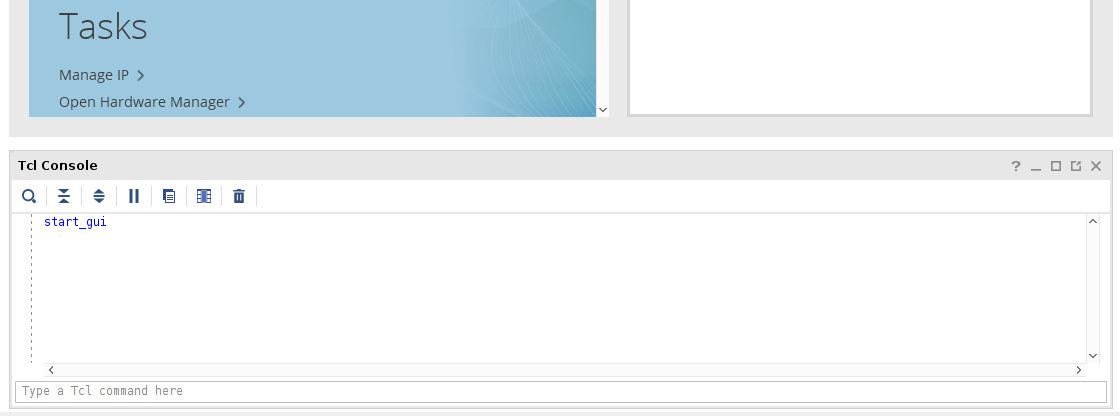
\includegraphics[width=0.9\textwidth]{images/viv_tcl_con.png}
    \caption{The TCL Console within the Vivado opening window}
    \label{fig:viv_tcl_con}
\end{figure}




\section{Creating a Vivado Project Using a Board File}
\label{sec:create_proj}
From the \textit{Getting Started} page, select \textbf{Create New Project}. In the \textit{Project Name} dialog box, type the project name and location; make sure to choose a directory to which you extracted the contents of the provided \textit{zip} file for this tutorial. In the \textit{Project Type} dialog box, select \textbf{RTL Project}. In the \textit{Add Sources} dialog box, ensure that the Target language is set to \textbf{Verilog}; we don't have any source to add to this project. We don't have anything to add in the \textit{Add Constrains and Add Existing IP} dialog box, since we are using a board file instead of a constraints file. Note, it is possible to use both a board file and a constraints file in the same project; details will be provided later in the tutorial. In the \textit{Default Part} dialog box, switch to the \textit{Boards} selection option at the top to choose from the installed board files. From the \textit{Vendor} drop-dwon menu, select \textbf{digilentinc.com}, and then select the \textbf{Nexsys4 DDR} option in the list (see Figure~\ref{fig:board_select} for reference). Click \textbf{Next} and then click \textbf{Finish} to finish creating the project.

\begin{figure}[!h]
    \centering
    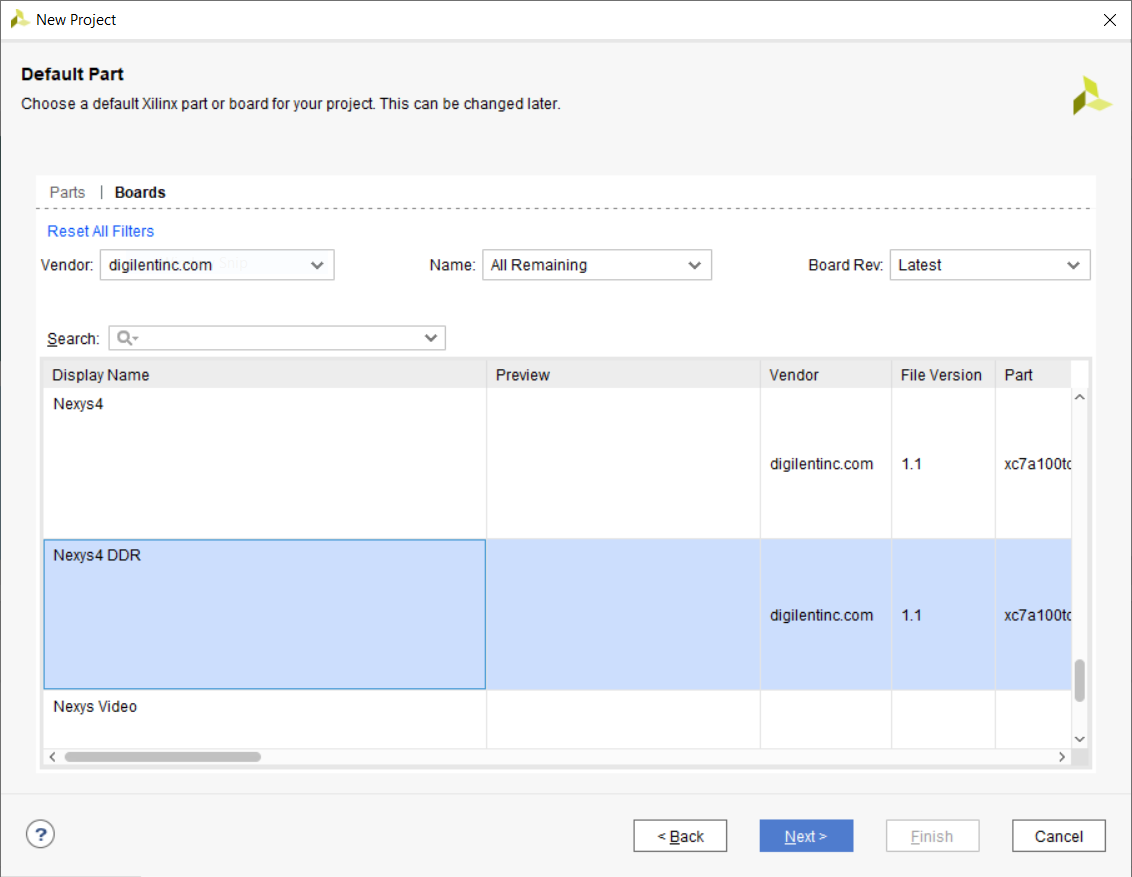
\includegraphics[width=0.9\textwidth]{images/board_select.png}
    \caption{The board selection dialog window}
    \label{fig:board_select}
\end{figure}

Follow the instructions from tutorial 2 to create a new \textit{Block Diagram} within your new Vivado project. In the block design editor, you should notice a new \textit{Board} tab within the sources window, as per Figure~\ref{fig:board_sources_tab}. This tab lists all of the interfaces defined within the board file. To connect something to one of these interfaces, double click the interface and select from the list of cores capable of connecting to that interface. While this way of connecting to the interfaces defined in the board file does work, it is more common to instantiate the core itself first, and then indicate that the core should be connected to the interface; we'll show how to do this later in the tutorial. If you don't know which cores are capable of connecting to the interfaces you'd like to use, this is a good way to find out. once an interface is connected, the icon beside the interface changes from unconnected~(\scalerel*{
\includegraphics{images/signal_unconnected.png}}{(})
to connected~(\scalerel*{
\includegraphics{images/signal_connected.png}}{(})
. if you think a signal should be connected but your project doesn't seem to be working, you can check this \textit{Board} tab to ensure the signal is being connected correctly.

\begin{figure}[!h]
    \centering
    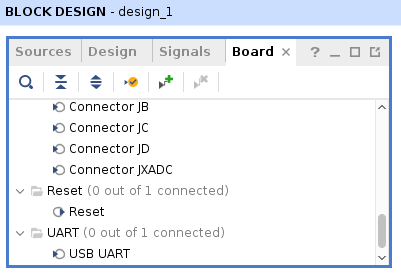
\includegraphics[width=0.5\textwidth]{images/board_sources_tab.png}
    \caption{The Board tab within the Block Design editor window}
    \label{fig:board_sources_tab}
\end{figure}




\section{Recreating the Simple MicroBlaze Project}
\label{sec:adding_cores}
We need to create the simple MicroBlaze project from tutorial 2 again, but there are some differences now that we are using a board file. Add the \textit{MicroBlaze} IP and click \textbf{Run Block Automation}, as we did in tutorial 2. Set the \textit{Local memory} to \textbf{32KB}, check the \textbf{Interupt Controller} option, and select the \textit{Clock Connection} option of \textbf{New Clocking Wizard (100 Mhz)}. Click \textbf{OK}. 

As with tutorial 2, we need to setup the \textit{Clocking Wizard} configuration to connect to the Nexsys board's clock pin. \textbf{Double click} the \textit{Clocking Wizard} to configure this core. you should notice a new tab called \textit{Board}; this tab allows you to connect the pins of this core to any compatible pins defined in the board file. For the input labelled \textit{CLK\_IN1}, use the drop-down menu to select \textbf{sys\_clock}. This will automatically connect that pin of the Clock Wizard core to the \textit{sys\_clock} pin defined in the board file. For the input labelled \textit{EXT\_RESET\_IN}, use the drop-down menu to select the \textbf{reset} pin. See Figure~\ref{fig:config_clock_wiz.png} for reference. If you go to the second tab of the configuration window, you should notice that Vivado automatically changed \textit{clk\_in1} to be a \textit{Single ended clock capable pin}, which we had to do manually in tutorial 2. In the \textit{Output Clocks} tab, the \textit{Reset Type} still needs to be modified to \textbf{Active Low}, since this is an output of the core and not specified by the board file (i.e. this is a user decision).

\begin{figure}[h]
    \centering
    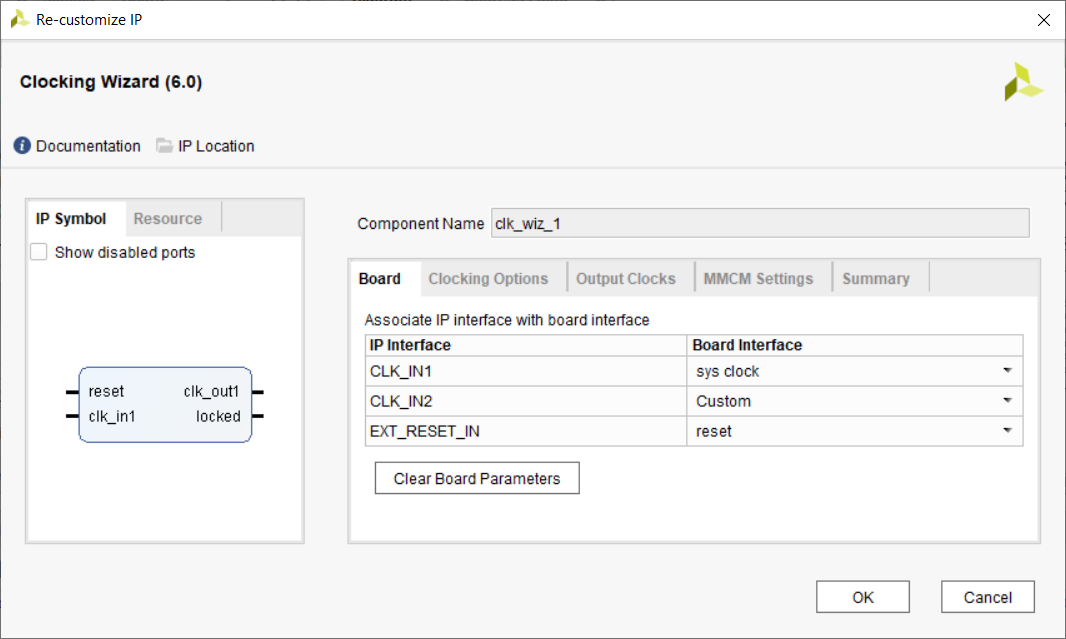
\includegraphics[width=0.9\textwidth]{images/config_clock_wiz.png}
    \caption{Clocking Wizard configuration dialog to select board file signals}
    \label{fig:config_clock_wiz}
\end{figure}

As with tutorial 2, the last step we need to do in order to make this a fully functional system is to connect the clock and reset signals to external ports. To do this, we'll use \textit{Connection Automation} again
(~\scalerel*{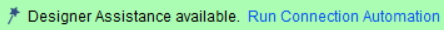
\includegraphics{images/connect_auto_pop.png}}{(}~). 
In the left pane, we see the clock and reset signals of the \textit{Clock Wizard}, and the ext\_reset\_n signal of the \textit{Processor System Reset} core. For each signal, there should be a drop down menu to select from compatible board file signals to connect to. In our case, each of these signals will have one option. Select the \textit{sys\_clock} signal for the clock input and the \textit{reset} signal for each of the reset inputs. Note that we don't have to indicate that the reset is \textit{Active Low} as we did in tutorial 2, since the board file has this information. Remember to actually tick the checkbox beside all the signals for which you want connection automation to run. See Figure~\ref{fig:conn_auto_clock2} for reference. We should now have a fully connected design.

\begin{figure}[h]
    \centering
    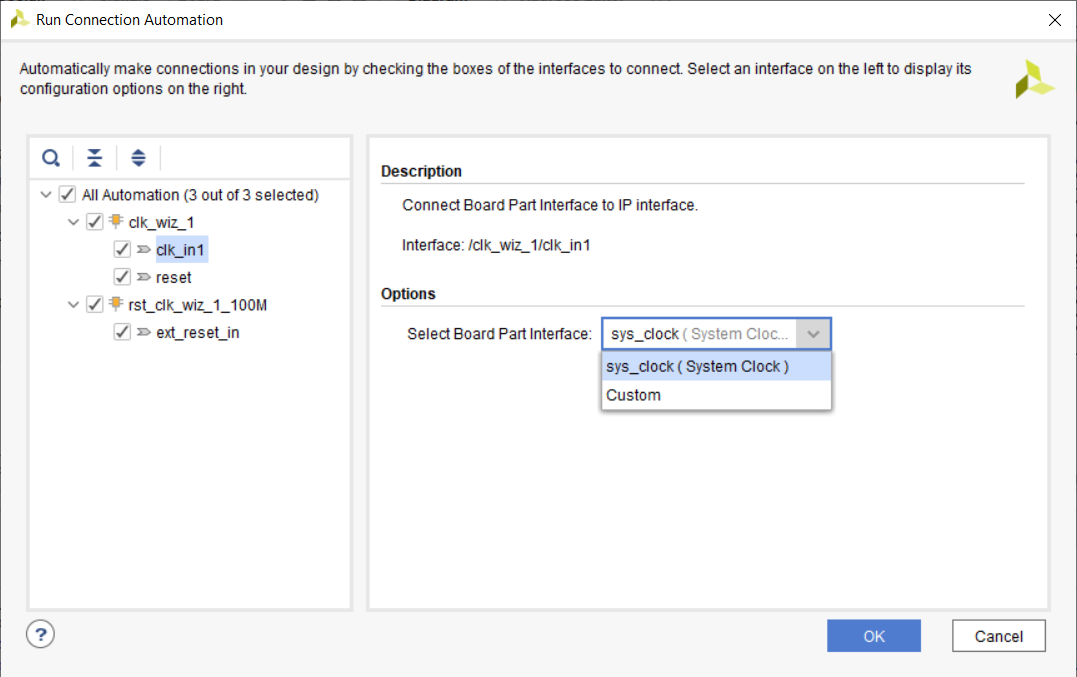
\includegraphics[width=0.9\textwidth]{images/conn_auto_clock2.png}
    \caption{Connection automation for the clocking wizard}
    \label{fig:conn_auto_clock2}
\end{figure}

Note, if you wanted to synthesize the design as is, you would need to connect something to the inputs of the \textit{Concat} block, otherwise you will get an error. A block that is commonly used to tie off unconnected signals is the the \textit{Constant} block, which simply has an output that is some constant value. We will be adding the UART core to use the interrupt, so there is no need for us to tie this signal to a constant value at this time.

To add the AXI Uartlite peripheral to our project, \textbf{Right click} anywhere in the block diagram, select \textbf{Add IP} and search for and select the AXI Uartlite. Connect the \textbf{interrupt} signal of the AXI Uartlite to the \textbf{In0} signal of \textit{Concat}, and configure the \textit{Concat} core such that it has no unconnected inputs (as in tutorial 2). Run \textit{Connection Automation} again to handle the remaining Uartlite signals. In the \textit{Connection Automation} window, select to run \textit{Connection Automation} for all signals by selecting all the check boxes in the left pane. Click the \textit{uart} signal specifically to see that the board signal for the \textit{usb\_uart} is automatically selected for that connection; if it is not, select it from the drop-down menu. See Figure~\ref{fig:conn_auto_uart} for reference.

\begin{figure}[h]
    \centering
    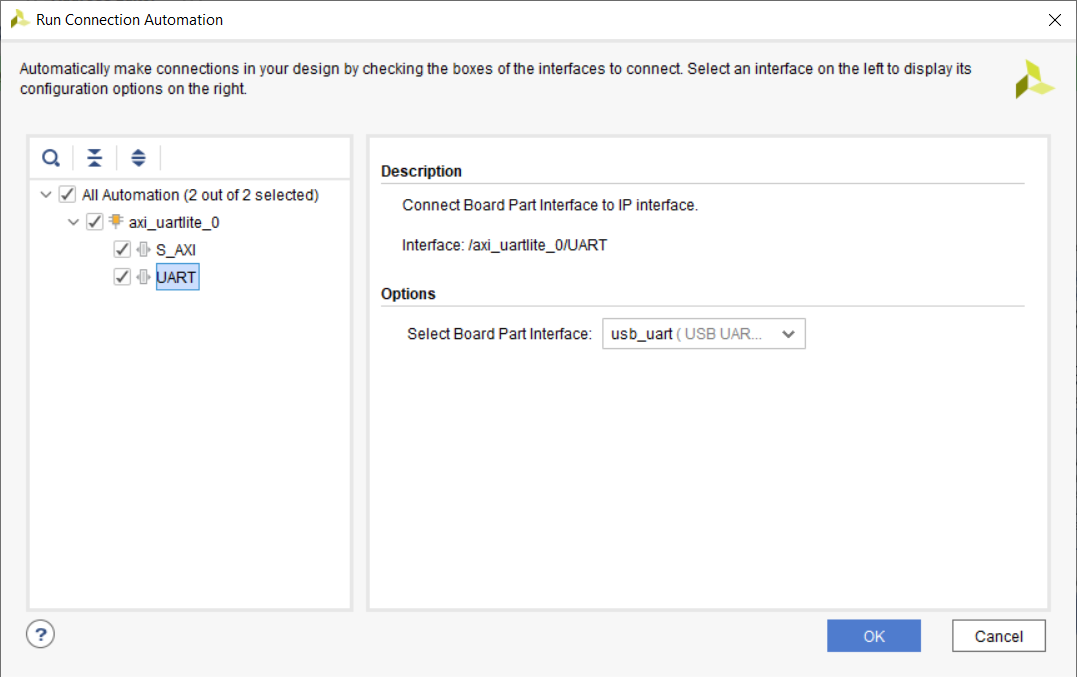
\includegraphics[width=0.9\textwidth]{images/conn_auto_uart.png}
    \caption{Connection automation for the uartlite}
    \label{fig:conn_auto_uart}
\end{figure}




\section{Adding an AXI BRAM Controller}
\label{sec:add_memory}
To add an AXI BRAM to the MicroBlaze project, \textbf{right click} anywhere in the block diagram, select \textbf{Add IP} and search for and select the \textit{AXI BRAM Controller}. Mdify the configuration of the BRAM controller by \textbf{double clicking} it to bring up the configuration window. We want to change the number of output BRAM interfaces to one, since we only need to interface with a single BRAM (See Figure~\ref{fig:bram_cntr_config} for reference). We can now run \textit{Connection Automation} again to finish the connectivity for the newly added BRAM. In the \textit{Connection Automation} window, select the check box to enable connection automation for all connections. Click on the \textit{BRAM\_PORTA} signal, and select \textbf{New Blk\_Mem\_Gen} in the \textit{Blk\_Mem\_Gen} pull-dwon menu. This will instruct \textit{Connection Automation} to create a new BRAM to connect the BRAM controller to. alternatively, you could have created a \textit{Block Memory Generator} core before running \textit{Connection Automation}. See Figure~\ref{fig:conn_auto_bram} for reference.

\begin{figure}[!h]
    \centering
    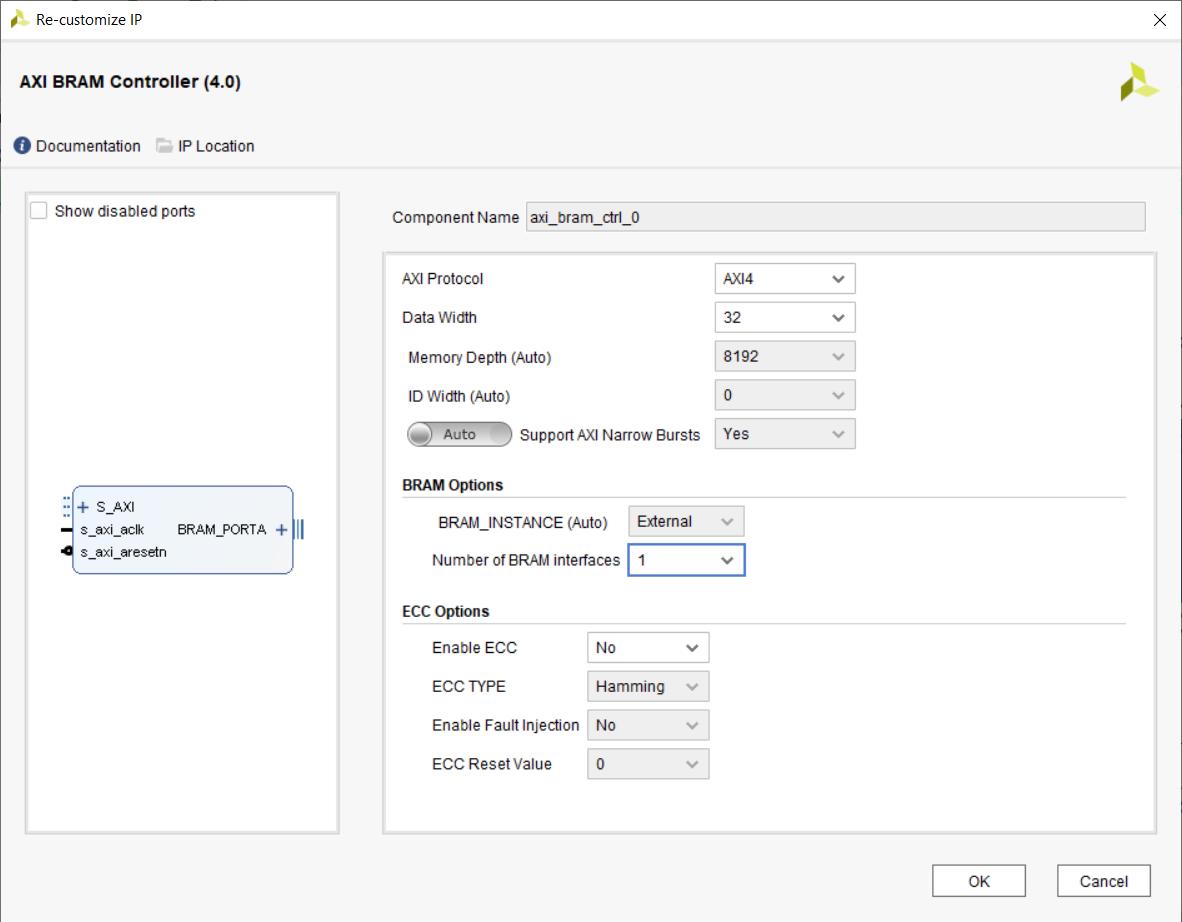
\includegraphics[width=0.84\textwidth]{images/bram_cntr_config.png}
    \caption{Configuration window for the AXI BRAM Controller}
    \label{fig:bram_cntr_config}
\end{figure}

\begin{figure}[!h]
    \centering
    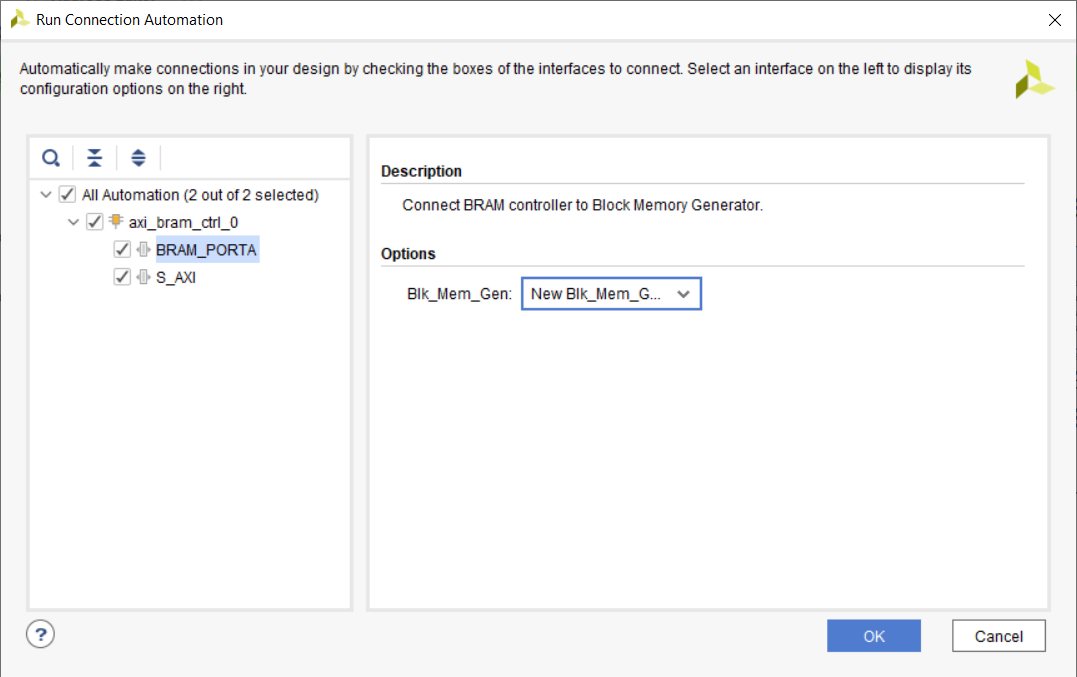
\includegraphics[width=0.84\textwidth]{images/conn_auto_bram.png}
    \caption{Connection automation for the AXI BRAM Controller}
    \label{fig:conn_auto_bram}
\end{figure}

By default, the generated BRAM is created with a size of 8KB. To increase the size of the BRAM open the \textit{Address Editor} view and expand the \textit{Data} section of the \textit{microblaze\_0} core (or whatever you happen to call your MicroBlaze instance). You can change the \textit{Range} pull-dwon menu for the \textit{axi\_bram\_ctrl\_0} entry to the size you'd like your BRAM to be. When the block diagram is synthesized, this \textit{Range} parameter is propagated to the BRAM core and the size is set automatically. Increase the size to 16K, see Figure~\ref{fig:address_edit_bram} for details.

\begin{figure}[h]
    \centering
    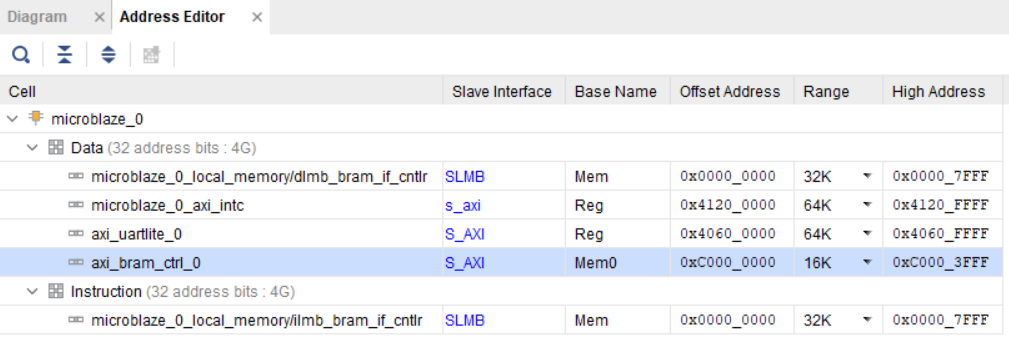
\includegraphics[width=0.9\textwidth]{images/address_edit_bram.png}
    \caption{Address Editor with Range field modified}
    \label{fig:address_edit_bram}
\end{figure}

Follow the steps for tutorial 2 to validate the block diagram, generate an HDL wrapper, ans synthesize, implement, and generate the bitstream for the design. Note, we don't need to check that the signal names in out wrapper match the names in our constraints file, since we don't have a constraints file. If, in a future project, you choose to connect some signals using the board file and some using a constraints file, you would need to check the top-level names of only those signals whose connections are not determined in the board files. Once the bitstream generation is complete, export the hardware and \textbf{Launch SDK} in order to test the system with software. When \textit{Vivado SDK} launches, create a \textit{Hello World} template program. Open the \textit{helloworld.c} source file and modify it's contents to that of Figure~\ref{fig:mem_app}. For more details on these steps, refer to the instructions in tutorial 2.

\begin{figure}[!h]
\centering
\begin{minted}
[
frame=lines,
framesep=2mm,
baselinestretch=1.2,
bgcolor=white,
fontsize=\footnotesize,
linenos,
breaklines,
]
{c}
#include <stdio.h>
#include "platform.h"
#include "xil_printf.h"
#include "xparameters.h"

#define MEMSIZE 16
volatile unsigned int* membase = (unsigned int*) XPAR_AXI_BRAM_CTRL_0_S_AXI_BASEADDR;

int main()
{
    int i, val, err = 0;
    
    init_platform();
    
    print("Writing to Memory\n\r");
    for(i = 0; i < MEMSIZE; i++)
    {
        *(membase+i) = i+1;
    }
    
    print("Reading from Memory\n\r");
    for(i = 0; i < MEMSIZE; i++)
    {
        val = *(membase+i);
        
        if(val != i+1) 
        {
            xil_printf("Error: at addr \%x, read \%d but expected \%d\n\r", membase+i, val, i+1);
            err = 1;
        }
    }
    
    if(!err)
    {
        print("No errors encountered\n\r");
    }

    cleanup_platform();
    return 0;
}
\end{minted}
\vspace{-0.7cm}
\caption{Modified Hello World application using BRAM memory}
\label{fig:mem_app}
\end{figure}

The application simply writes to the BRAM memory with increasing values and then reads back the values to make sure the writes were performed correctly. Note, the macro:

\begin{verbatim}
    XPAR_AXI_BRAM_CTRL_0_S_AXI_BASEADDR
\end{verbatim}

\noindent
is defined automatically in the file \textit{xparameters.h}, though make sure to check that file to ensure the macro has the same name. This program also uses the function \textit{xil\_printf}, which is a Xilinx version of the printf function. The \textit{xil\_printf} function has smaller memory footprint than the actual printf function, though it doesn't support floating point numbers. In some cases, applications we develop (if you want to use the full printf function for example) will be too large to fit into the instructions memory created when you ran \textit{Block Automation} to create your MicroBlaze project. In this case, we'll need to change the linker script in order direct the assembler to store the code in a different memory. Now that we've added a memory, we can demonstrate that feature.

\textbf{Right Click} on your project name in the left pane and select \textbf{Generate Linker Script}; the window that appears is shown in Figure~\ref{fig:gen_linker_script}. On the left side is listed the various memories connected to your MicroBlaze, and on the right side we see the various parts of the program that we can assign to be stored in particular memory devices. Select the drop-down menu labelled \textit{Place Data Sections in} and note that we have the BRAM controller listed here. If you select the drop-down menu labelled \textit{Place Code Sections in}, you won't see the BRAM controller. This is because the BRAM Controller is only connected to the Data AXI interface in our original project, so the instruction port of the MicroBlaze cannot access our BRAM. We don't need to change the linker script at this, so simply press \textbf{Cancel}. These steps were simply to show you how you would move sections of the program to different memories for future projects. Note, the \textit{Heap} is used for dynamic memory allocation, so if some program you are writing is running out of working memory, moving the heap to a larger memory should alleviate this problem.


\begin{figure}[h]
    \centering
    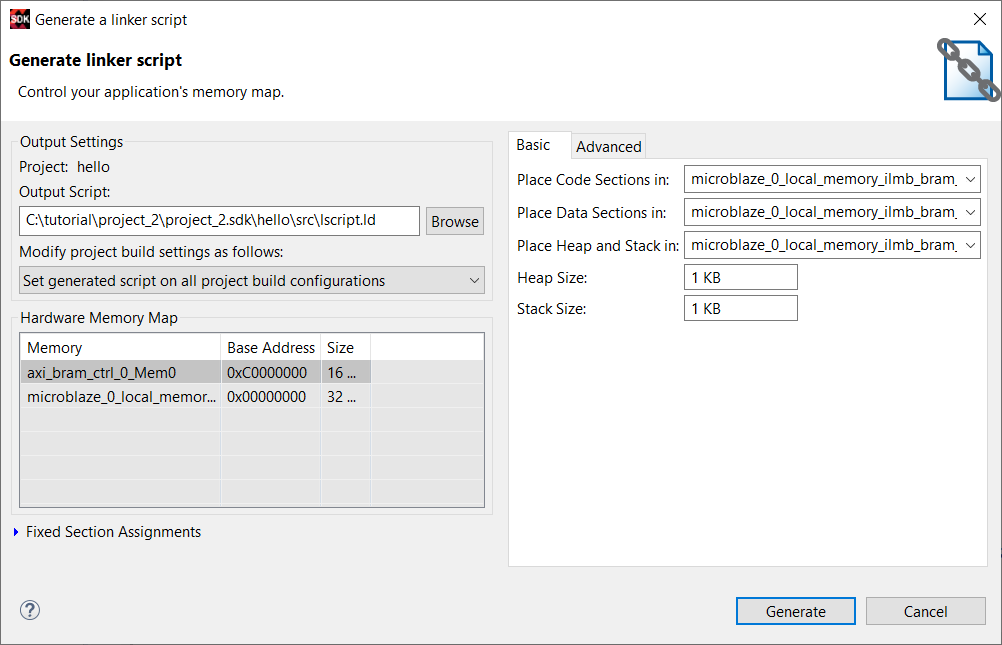
\includegraphics[width=0.8\textwidth]{images/gen_linker_script.png}
    \caption{Generate Linker Script dialog}
    \label{fig:gen_linker_script}
\end{figure}

Generate a \textit{Run Configuration}, connect to the \textit{UART Terminal}, and then run the program on the Nexsys board, based on the instructions from tutorial 2. Verify that we see the expected output. Next, create a \textit{Debug Configuration} and run the application in debug mode, again based on the instruction from tutorial 2. Select \textbf{Yes} when it asks you to change to the \textit{Debug perspective}. recall from tutorial 2 that this debug console implements the debug features of the gdb debugger. 

In regards to memory, one useful debug feature is the ability to add a memory monitor. Click on the memory tab in the lower right corner of the \textit{Debug perspective}. If the memory tab isn't visible, go to \textbf{Window $\rightarrow$ Show View $\rightarrow$ Memory} to open the view. In the memory pane, click the + sign to add a \textit{Memory Monitor}. In the dialog box that comes up, enter \textbf{brambase} and press \textbf{OK}~(see Figure~\ref{fig:add_mem_mon} for reference). Now add some breakpoints to the code and run the program to watch the memory change as the writes to \textit{brambase} are encountered in the code. This is a useful way to examine the contents of memory to debug your code.

\begin{figure}[h]
    \centering
    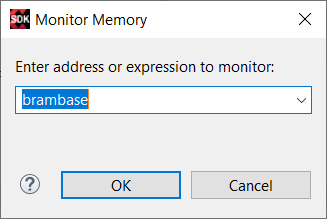
\includegraphics[width=0.4\textwidth]{images/add_mem_mon.png}
    \caption{Adding a memory monitor in the GDB debug view}
    \label{fig:add_mem_mon}
\end{figure}




\section{Adding an AXI DDR Controller}
\label{sec:add_ddr}
We want to replace the AXI BRAM controller we added to the project with an AXI DDR controller, to allow us to access the DDR memory on the Nexsys board. \textbf{Close} the Vivado SDK and reopen the block diagram containing your MicroBlaze project. Delete the \textit{AXI BRAM Controller} and the \textit{Block Memory Generator} from the design. \textbf{Right click} anywhere in the diagram and select \textbf{Add IP}. Search for the \textit{Memory Interface Generator (MIG) peripheral} and add that core to your project. Press \textbf{Run Block Automation} and select to run \textit{Block Automation} on the \textit{mig\_7series\_0} core that was just added to your project. Error [BD 41-1273] may appear during automation, but can be safely ignored. The block automation used the data in the board file to set the configuration details for the memory controller. If you open the configuration window for the \textit{MIG} (by double-clicking) and step through the panes of the configuration, you'll note that there are a lot of configuration options for the memory controller. In fact, the \textit{MIG} even requires all the pin locations to be entered by hand. Using the board file saves us this hassle. Make sure not to change any of the settings while you look at the configuration panes of the \textit{MIG}.

To connect the \textit{MIG} to the MicroBlaze, click \textbf{Run Connection Automation}. Select all of the check-boxes for the \textit{MIG} signals except for the \textit{sys\_clk\_i} signal; the connection automation tries to connect this signal to the output of the \textit{Clocking Wizard}, which generates errors later in the project flow. Once the connection automation has finished, manually connect the \textit{sys\_clk\_i} signal to the \textit{sys\_clock} siganl used as the input to the \textit{Clocking Wizard}. Open the \textit{Address Editor} and examine the newly added entry for the \textit{MIG}; the \textit{MIG} has been allocated a memory space of size 128M, which corresponds to the size of the DDR chip connected to the FPGA on the Nexsys board. Select the \textbf{DDR2} bus on the memory controller, right click and select \textbf{Make External}, to propagate these signals to the pins of the FPGA.

As a final step, we'll modify the MicroBlaze such that the instruction port of the processor can access the AXI interface as well. Note, our program from before was small enough to fit in the BRAM, but we include these steps here as they may be useful for future projects in which the application cannot fit in the BRAM. \textbf{Double Click} the MicroBlaze to bring up its configuration window. Advance to the fourth page and select \textbf{Enable Peripheral AXI Instruction Interface} (see Figure~\ref{fig:uB_add_instr_axi} for reference). Press \textbf{OK} to enact the change. You'll notice that a second AXI port appeared on the MicroBlaze processor. To connect this port, run \textbf{Connection Automation} once again. The \textit{AXI Interconnect} will be automatically modified to include 2 AXI master ports, with both the data and instruction port from the MicroBlaze connected.

\begin{figure}[h]
    \centering
    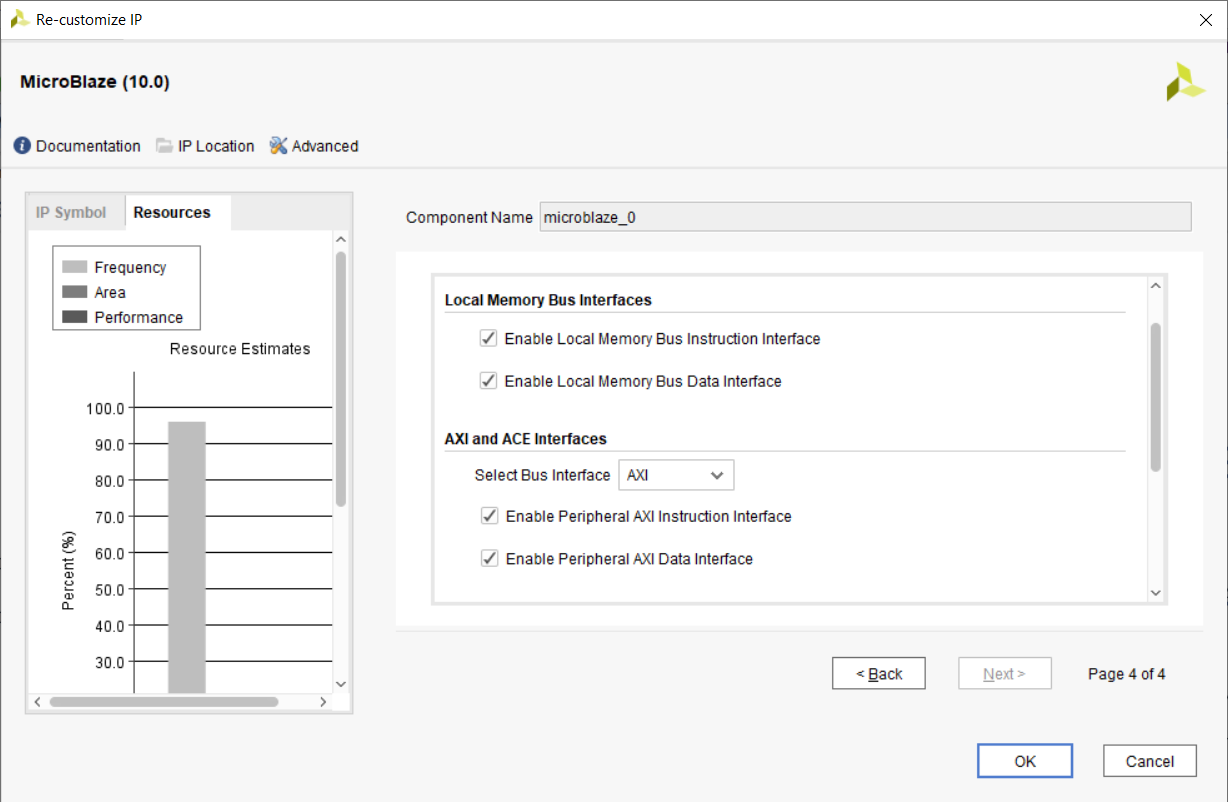
\includegraphics[width=0.8\textwidth]{images/uB_add_instr_axi.png}
    \caption{Reconfiguring the MicroBlaze to support AXI for instructions}
    \label{fig:uB_add_instr_axi}
\end{figure}

Now that we've added the MIG and reconfigured the MicroBlaze, validate the deign and then synthesize, implement, and generate the bitstream for the project. Once the project is done building, export the hardware and launch the \textbf{Vivado SDK}. See tutorial 2 for details. Once the \textit{Vivado SDK} window comes up, open the helloworld example that we created earlier and change the contents of the \textit{helloworld.c} file to reflect the changes in Figure~\ref{fig:mem_app2}.

\begin{figure}[!h]
\centering
\begin{minted}
[
frame=lines,
framesep=2mm,
baselinestretch=1.2,
bgcolor=white,
fontsize=\footnotesize,
linenos,
breaklines,
]
{c}
#include <stdio.h>
#include "platform.h"
#include "xil_printf.h"
#include "xparameters.h"

#define MEMSIZE 16
volatile unsigned int* membase = (unsigned int*) XPAR_MIG_7SERIES_0_BASEADDR;

int main()
{
    int i, val, err = 0;

    init_platform();

    print("Writing to Memory\n\r");
    for(i = 0; i < MEMSIZE; i++)
    {
        *(membase +i) = i+1;
    }

    print("Reading from Memory\n\r");
    for(i = 0; i < MEMSIZE; i++)
    {
        val = *(membase+i);

        if(val != i+1)
        {
            xil_printf("Error: at addr \%x, read \%d but expected \%d\n\r", membase+i, val, i+1);
            err = 1;
        }
    }

    if(!err)
    {
        print("No errors encountered\n\r");
    }

    cleanup_platform();
    return 0;
}
\end{minted}
\vspace{-0.7cm}
\caption{Modified Hello World application using DDR memory}
\label{fig:mem_app2}
\end{figure}

\noindent
The primary change made is the updating of line~7 with the base address of the \textit{MIG}:

\begin{verbatim}
    XPAR_MIG_7SERIES_0_BASEADDR
\end{verbatim}

\noindent
This macro is now defined in the \textit{xparameter.h} file of the \textit{board support package}, which was updated when we reexported the hardware for our newly updated bitstream. \textbf{Run} the \textit{Run Configuration} that we already created earlier in the tutorial and observe the output printed to the console (make sure to connect to the UART device from the SDK Terminal tab first). We should see the output \textit{No errors encountered}. Also, rerun the \textit{Debug Configuration} and verify that you can add a \textit{Memory Monitor} for ddr based memories as well. \textbf{Add} a \textit{Memory Monitor} for address \textit{membase}, \textbf{add} a breakpoint right before the write to \textit{membase}, and then step through the program to see the memory change one entry at a time. 




\section{Summary}
\label{sec:summary}
MicroBlaze systems often need to connect to memories other than the primary data and instruction memory created by the \textit{Block Automation} tool. The AXI protocol is generally used to facilitate this connection, and Vivado has AXI-based controllers for both the BRAM memory within the FPGA and the DDR memories often connected to the pins of the FPGA. The MicroBlaze project was augmented with both of these types of memories, and an example program was developed that could write and read from these two types of memories. The use of \textit{board files} greatly eased this process, as it included both the pin constraints for all external pins we needed to use, removing the need for an \textit{xdc} file, and the configuration details for the DDR2 memory.



%\newpage
%S\printbibliography

\end{document}
